\chapter{Interpolation, Root Finding and Minimization}
\label{sec:interpolation}

In this Chapter some very important mathematical tools will be reviewed. These will be intensively used later on throughout the book.

\section{Linear Interpolation}
\label{linear-interpolation}

Consider to have recorded the value of a quantity at three points in time as in Fig.~\ref{fig:samples_for_interpolation}.
Starting from this small data sample we can infer the value of this quantity at different times using the \emph{interpolation} technique. Clearly this is 
possible only under certain assumptions that will be described along with the example.

\begin{figure}[htbp]
  \centering
  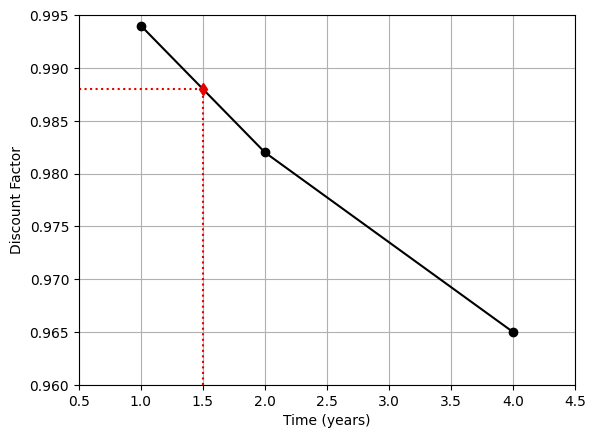
\includegraphics[width=0.7\textwidth]{figures/interp_example1}
  \caption{Plot of the discount curve described in the text.}
  \label{fig:samples_for_interpolation}
\end{figure}

Given two sample points $d_1$ and $d_2$ taken at two different times $t_1$ and $t_2$ a new value, between these two, can be found as the point lying on the 
\textbf{line} connecting $d_1$ and $d_2$ at the desired time. Here the main assumption is that the quantity is changing \textbf{linearly} with the time in the
interval $[t_1, t_2]$.

\begin{attention}
\subsubsection{Derivation}
The equation of a line for two points $(t_1, d_1)$ and $(t_2, d_2)$ can be written as:

\begin{equation}
\frac{t - t_1}{t_2 - t_1} = \frac{d - d_1}{d_2 - d_1}
\end{equation}

Setting $w = \cfrac{t - t_1}{t_2 - t_1}$ and solving for $d$ we find the desired solution:

\begin{equation}
(d_2 - d_1)\cdot w = d - d_1\quad\implies\quad d = (1 - w)\cdot d_1 + w \cdot d_2
\end{equation}

This formula can be interpreted as a weighted average where the weights are inversely related to the distances from the end points to the unknown 
point ($w_1 = (1 - w) = \cfrac{t_2 - t}{t_2 -t_1}, w_2 = w$), which means that the closer point has more "influence" than the farther point on the result.
\end{attention}

Although quite simple, you don't need to implement the interpolation formula from scratch, instead it can be used the one provided in 
\texttt{scipy.interpolate.interp1d}. 

\pythoncodenon{code/discount_1.py}

\begin{ioutput}
0.988
\end{ioutput}

\emph{Always interpret critically your results to guess if they make sense or not and avoid mistakes}. In the previous example we certainly expected 
something between 0.994 and 0.982 (our range ends) furthermore since we are looking for the discount factor at a time which is halfway the considered 
interval, the result will be somehow in the middle of $d_1$ and $d_2$. This simple kind of reasoning should be applied every time you have a result to 
quickly judge it.

\begin{curiosity}
\subsubsection{Epic Failure}
The Mars Climate Orbiter \emph{was} a 638~kg (1,407~lb), 326.7~M\$ space probe launched by NASA on December 11, 1998 to study Martian climate, atmosphere, 
and surface changes. 

On September 15, 1999, the necessary corrections to speed and direction of the probe were computed in order to place the spacecraft at an optimal position 
for an orbital insertion maneuver that would bring it around Mars at the proper altitude. 
But one week later communication with the spacecraft was permanently lost as it went into Martian orbital insertion. 

A committee of experts was created to investigate the reasons of 
such failure and they found out that the spacecraft encountered Mars at a lower than foreseen altitude causing either its destruction by atmospheric 
friction or making it bouncing against the atmosphere re-entering heliocentric orbit after leaving Mars.

The primary cause of this discrepancy was found in one piece of software (supplied by Lockheed Martin) that produced results in "Imperial" units, 
while a second system (supplied by NASA) expected those results to be in SI units. Specifically, the software calculated the total impulse produced by 
thrust in \emph{pound-force seconds}. The trajectory calculation software then used these results, expected to be in \emph{newton seconds}, thus 
incorrect by a factor of 4.45, to update the predicted position of the spacecraft.
	
NASA took the entire responsibility for having vaporized about 300~M\$ in the Martian atmosphere, mainly for failing to make the appropriate checks and 
tests that would have caught this unit discrepancy~\cite{bib:mars}.	
\end{curiosity}

\subsubsection{Extrapolation Risk}

Interpolation is primarily designed to estimate values \textbf{within} the range of known data points. Attempting to extrapolate beyond the data range 
can lead to inaccurate results and is generally discouraged. Extrapolation assumes that the relationship between data points remains constant \emph{also} outside 
the known range, which may not be valid in general.

\subsection{Log-linear Interpolation}
\label{log-linear-interpolation}

When there is an exponential relationship between the two variables (e.g. $t$ and $p$) we can fall back to the linear case by a simple variable transformation. 
Imagine that $p=e^{-rt}$, applying the logarithm to both sides of the equation gives:

\begin{equation}
f = \log(p) = \log(\exp(-rt)) = -rt
\end{equation}
so there is a linear relation between the new variable $f$ and $t$. At this point we can use the results of the previous Section to interpolate for values of 
$f$, just remember to exponentiate the final result to get the correct value of $p$.

\pythoncodenon{code/discount_1.1.py}

\begin{ioutput}
0.988
\end{ioutput}

\subsection{Limitations of Interpolation}
Interpolation is just an approximation and works well when we are trying to apply it between two points that are close enough to believe that the function is 
almost linear in that interval.

It can be easily demonstrated that the linear approximation between two points of a given function $f(x)$ gets worse with the second derivative of the approximated function ($f''(x)$). This is intuitively correct: the "curvier" the function, the worse the approximation made with simple linear interpolation, see Fig.~\ref{fig:sine_interp} where we try to interpolate a sine function.

\begin{figure}
  \centering
  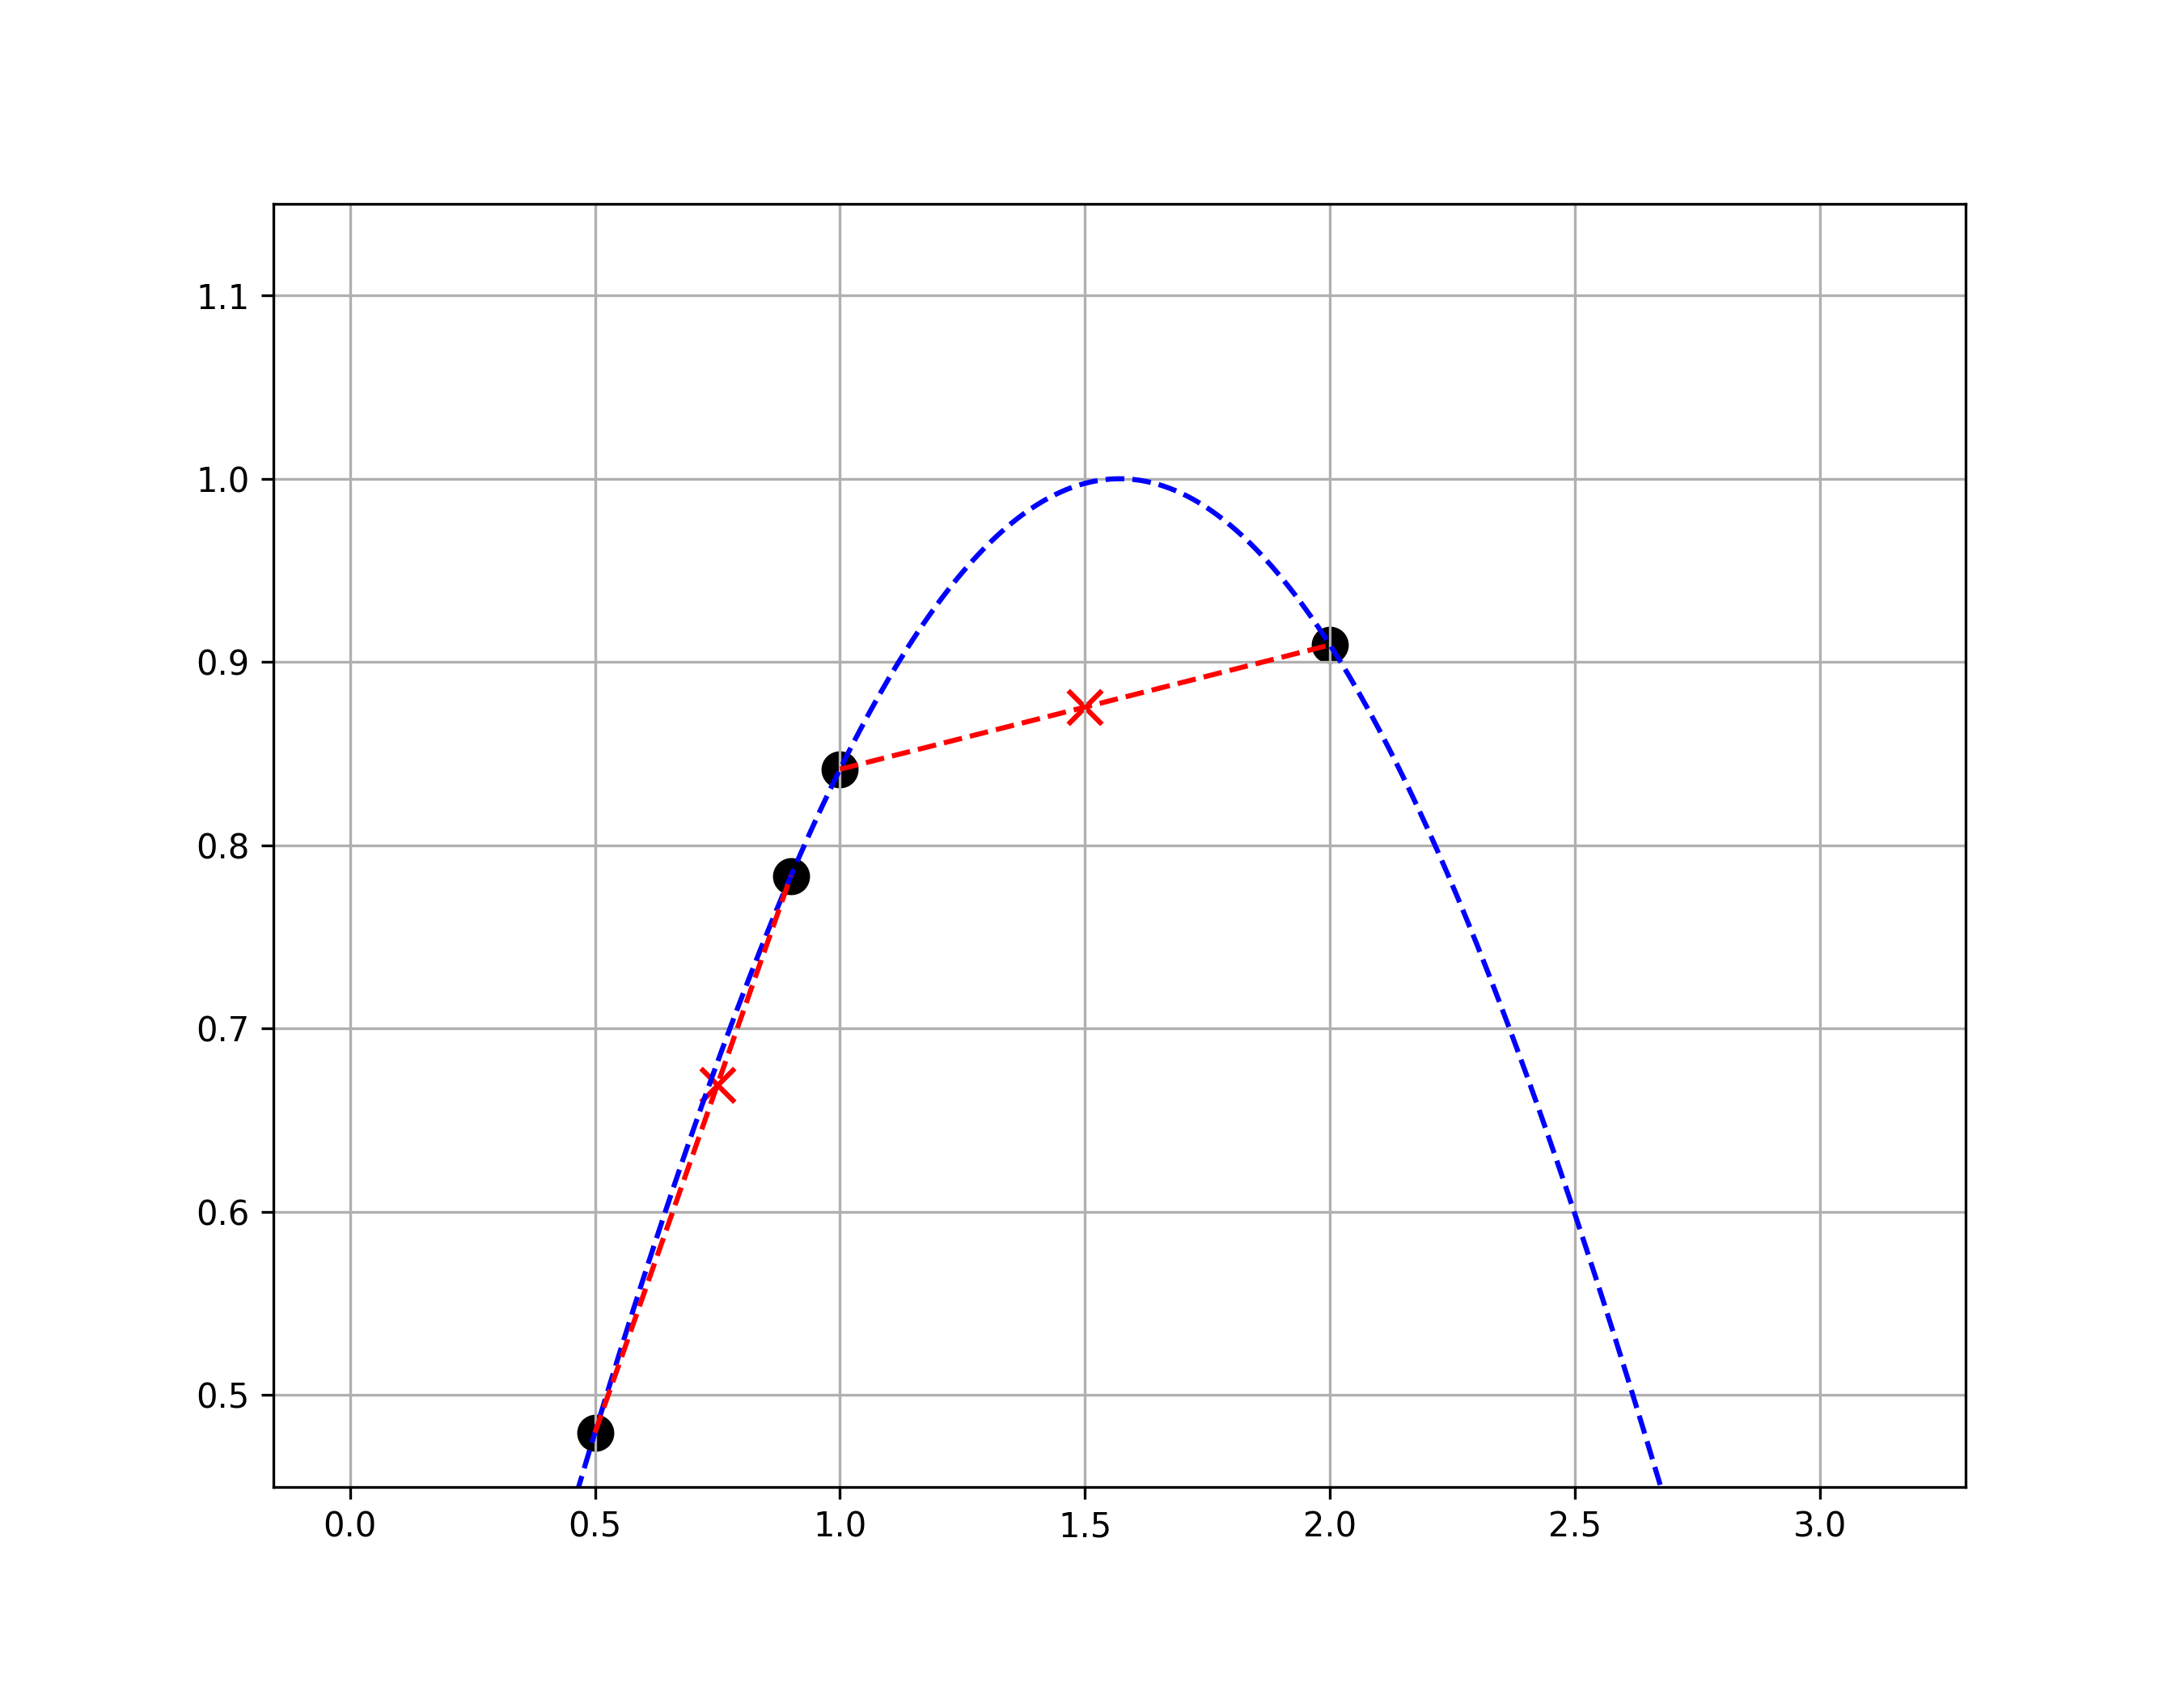
\includegraphics[width=0.7\textwidth]{figures/wrong_interp.png}
  \caption{Trying to approximate a sine function with a line is clearly not going to work unless the interpolation interval is very small.}
  \label{fig:sine_interp}
\end{figure}

To improve the approximation accuracy with complicated curves e.g. in the evaluation of natural logarithm or trigonometric functions, a higher order polynomial 
can be used ($p(x)=a_0 + a_1\cdot x + a_2\cdot x^2+\cdots$). It has to be clear however that going to higher degrees does not always help~\cite{bib:runge}.
Some interpolation methods, indeed, can result in \emph{overfitting}. This means the interpolating function fits the data points very closely but may not 
generalize well to unseen data, i.e. it can lead to excessive fluctuations between data points.

\section{Root Finding}
\label{sec:root_finding}

To find the zeros of a function $f(x)$ means to determine the values $\hat{x}$ such that $f(\hat{x})=0$ and the process is equivalently called finding the 
roots of $f(x)$. There are various methods to achieve that, in the following we will see few of them.

\subsection{Bisection}
\emph{Bisection}~\cite{bib:bisection} method is considered the simplest one-dimensional root-finding algorithm.
Suppose we know two points of an interval $[a,b]$, and that $f(a)< 0$ and $f(b)> 0$.
Since the value of $f(a)$ is negative and $f(b)$ is positive, the bisection method assumes that the root $x$ lies somewhere between $a$ and $b$.

Taking the midpoint of this $[a, b]$ interval as $c$, the algorithm evaluates the value $f(c)$.
If $f(c) = 0$ or is very close to zero by some predetermined error tolerance value, then a root is declared as found. If $f(c)< 0$, then we may conclude that a root exists along the interval $[c, b]$, or along $[a,c]$ otherwise.

On the next evaluation, $c$ is replaced as either $a$ or $b$ accordingly. With the new interval shortened, the bisection method repeats with the same evaluation to determine the next value of $c$. This process continues, shrinking the width of the interval until the root is determined as found. Figure~\ref{fig:bisection} shows an example of bisection algorithm application.

\begin{figure}[htbp]
\centering
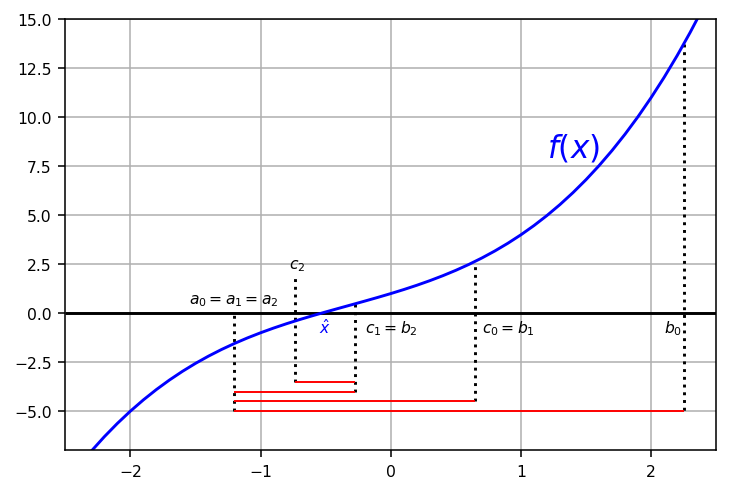
\includegraphics[width=0.7\linewidth]{figures/bisection}
\caption{Example of bisection algorithm to find the roots of a function $f(x)$.}
\label{fig:bisection}
\end{figure}

The biggest advantage of the bisection method is it is guaranteed to converge to an approximation of the root, given a predetermined error tolerance level 
and the maximum number of iterations allowed. It should be noted that the bisection method does not require knowledge of the derivative of the unknown 
function. In certain continuous functions, the derivative could be complex or even impossible to calculate. This makes this method extremely valuable for 
working on functions that are not smooth.
Contrary, its major drawback is that it takes up more computational time in the iterative evaluation as compared to other root-finder methods. 

Although this method is simple enough to be quickly implemented in \texttt{python} we will opt for the surely bug free version available as 
\texttt{scipy.optimize.bisect} (for the usage of \texttt{args} see Section~\ref{sec:kwargs_args}).

\begin{ipythonnon}
from scipy.optimize import bisect 

def f(x, a, b, c):
    return a*x**2 + b*x + c 
  
print (bisect(f, -3, 3, args=(1, -8, 4)))
\end{ipythonnon}
\begin{ioutput}
0.5358983848632306
\end{ioutput}

An alternative algorithm is the \emph{Brent's method}~\cite{bib:brent} which combines the advantages of both bisection and secant 
(another root-finding algorithm) methods. Its \texttt{python} implementation is \texttt{scipy.optimize.brentq}.

\begin{ipythonnon}
from scipy.optimize import brentq
    
print (brentq(f, -3, 3, args=(1, -8, 4)))
\end{ipythonnon}
\begin{ioutput}
0.5358983848622614
\end{ioutput}

\noindent
The results match down to the eleventh digit.

\subsection{Newton-Raphson Method}

Newton's method, also known as the Newton-Raphson method, is a root-finding algorithm which produces successively better approximations to the roots (or zeroes) 
of a real-valued function. 
%The most basic version starts with a real-valued function f, its derivative f′, and an initial guess x0 for a root of f. If f satisfies certain assumptions and the initial guess is close, then

The idea is to start with an initial guess $x_0$, then to approximate the function by its tangent line ($g(x)$), 
\begin{equation*}
g(x) = f(x_0) + \cfrac{\partial f}{\partial x}(x_0)(x - x_0)
\end{equation*}
and finally to compute the $x$-intercept of this tangent line. This $x$-intercept will typically be a better approximation to the original function's root 
than the first guess, and the method can be iterated.

Suppose the tangent line to the curve $f(x)$ at $x = x_n$ intercepts the $x$-axis at $x_{n+1}$ then we have two cases:
\begin{enumerate}
\item the original function value in $x_{n+1}$ is "close enough" to 0 such that we are happy with this approximate solution e.g.
\begin{equation*}
f(x_{n+1}) < \texttt{tol}=10^{-8}
\end{equation*}
where the parameter \texttt{tol} is set in advance. In this case we are done and the algorithm stops;
\item otherwise we need to solve for $x_{n+1}$ and iterate the process again. Indeed 
\begin{equation*}
g(x_{n+1}) = f(x_n) + \cfrac{\partial f}{\partial x}(x_n)(x_{n+1} - x_n) = 0
\end{equation*}

from which we get
\begin{equation*}
f(x_{n})-0 = f'(x_n)(x_{n}-x_{n+1}) \Rightarrow x_{n+1}=x_n-\frac {f(x_n)}{f'(x_n)}
\end{equation*}

Another iteration is then started from $x_{n+1}$.
\end{enumerate}

The method will usually converge, provided this initial guess is close enough to the unknown zero, and that $f'(x_0) \neq 0$.
\begin{center}
	\includegraphics[width=0.6\linewidth]{figures/newton_method}
\end{center}

\begin{ipythonnon}
from scipy.optimize import newton 

def f(x, a, b, c):
    return a*x**2 + b*x + c 
  
print (newton(f, 1, args=(1, -8, 4)))
\end{ipythonnon}
\begin{ioutput}
0.5358983848622547
\end{ioutput}

\section{Minimization  Algorithm}
\label{minimization-algorithm}

Minimization algorithms are fundamental tools across various scientific and engineering disciplines, playing a crucial role in finding the best possible 
solutions to problems by systematically reducing a defined \emph{objective function}. Whether it's minimizing energy in physics, cost in economics, 
error in machine learning models, or resource usage in operations research, these algorithms iteratively search through a solution space to locate the point 
that yields the smallest value of the function being optimized. 

Their importance lies in enabling us to automate the process of finding optimal or near-optimal solutions to complex problems that would be intractable to 
solve manually, leading to more efficient processes, better predictions, and improved designs.

\subsection{The Algorithm}
The minimization algorithm follows these steps:

\begin{itemize}
\tightlist
\item
  define an \emph{objective function} i.e. the function that has to be minimized;
\item
  set the initial value of the unknown parameters ($\mathbf{x_0}$) and their range of variability (those are the parameters that will be changed to find 
  the objective function minimum);
\item
  compute the objective function value;
\item
  move the parameter values to find a smaller value of the objective function (e.g. following the derivative direction w.r.t. each parameter); in 
  case constraints are defined, they will be considered when the parameter values are varied;
\item
  repeat the previous two steps until further variations of $\mathbf{x}$ won't change significantly the objective
  function (i.e. we have found a minimum of the function so the minimization process is completed !).
\end{itemize}

Let's see with a couple of examples how minimization can be implemented in \texttt{python} using the function \texttt{scipy.optimize.minimize}.

\subsubsection{Reducing the Production Costs}
\label{example}

In this exampe we will try to determine the optimal size of a circular cylindrical can of volume, $330~\mathrm{cm}^3$, that minimizes the cost of manufacture, 
see Figure~\ref{fig:cylinder}.

\begin{figure}[ht]
\centering
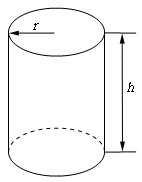
\includegraphics[width=0.2\textwidth]{figures/cylinder.png}
\caption{Graphical representation of the \emph{can} minimization example.}
\label{fig:cylinder}
\end{figure}

Clearly to minimize the costs, you need to reduce the amount of aluminum used, consequently the can surface. 
The objective function is given by the area of a cylinder

\begin{equation} 
S = 2\pi rh + 2\pi r^2 
\label{eq:can_surface}
\end{equation}
On the other hand the can volume is fixed to 33~cl or 330~$\mathrm{cm}^3$ and this allows to simplify the previous equation by removing $h$

\begin{equation*} 
V = \pi r^2 h = 330\quad\implies h = \cfrac{330}{\pi r^2}
\end{equation*}
Replacing $h$ in Eq.~\ref{eq:can_surface} 

\begin{equation}
S = 2\pi rh + 2\cdot(\pi r^2) = \cfrac{2\cdot 330}{r} + 2\cdot(\pi r^2)
\end{equation}
The objective function depends on one parameter only \texttt{x[0]} which is the can radius. We are going to use a \texttt{list} (or a \texttt{numpy.array}) 
even in this simple case so that the same code can be generalized to more complex problems with a larger number of parameters to minimize. 

\pythoncodenon{code/bootstrap_5.py}

Set the limits to our unknown variable and its initial value and finally run the minimization.

\begin{ioutput}
      fun: 264.356810914805
 hess_inv: <1x1 LbfgsInvHessProduct with dtype=float64>
      jac: array([5.68434189e-06])
  message: b'CONVERGENCE: NORM_OF_PROJECTED_GRADIENT_<=_PGTOL'
     nfev: 24
      nit: 9
   status: 0
  success: True
        x: array([3.7449385])
\end{ioutput}

Printing the result gives us the a lot of information about the minimization just performed, the most useful are:
\begin{itemize}
\item \texttt{func}: the objective function value at the last iteration;
\item \texttt{message}: the summary message (if it is \texttt{CONVERGENCE} is almost always OK);
\item \texttt{success}: the name is self explanatory;
\item \texttt{x}: the vector of unknown parameters that have been optimized.
\end{itemize}

Referring to Fig.~\ref{fig:minimization_diagnostic} it can be understood how minimization works. On the left plot it is shown the objective function value at 
each iteration, on the right the objective function vs the can radius is plotted.
The parameter $x[0]$ starts with the initial value we have set (1) then it is moved, too far, to 100.0 and indeed the evaluation gives an even higher value. 
$x[0]$ is then "adjusted" to $19.4\rightarrow 6.6\rightarrow 4.3\rightarrow 3.9\rightarrow 3.72\rightarrow 3.74\ldots$ always reducing the objective 
function value. Notice that the parameter is always moved according to the objective function derivative $\cfrac{dS}{dr}$ though by different amount.
Also the surface is a quadratic function of the radius so it is guaranteed to have just one minimum.

\begin{figure}[htb]
	\centering
	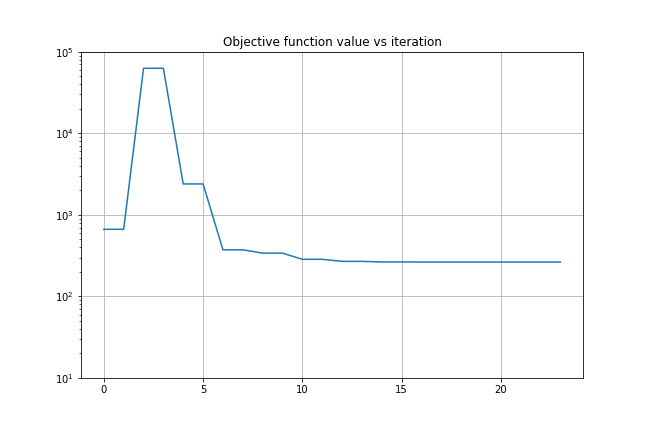
\includegraphics[width=0.45\linewidth]{figures/objective_function_value}
	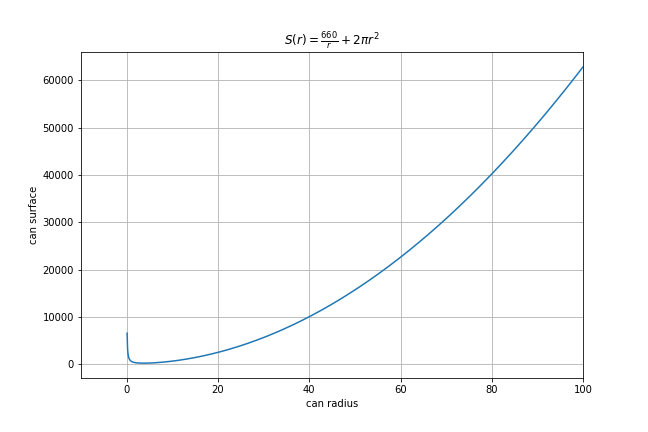
\includegraphics[width=0.45\linewidth]{figures/can_surface}
	\caption{Diagnostic plots for the minimization algorithm. On the left the objective function value at each iteration, on the right the objective function 
  value versus the can radius $x_0$.}
	\label{fig:minimization_diagnostic}
\end{figure}

Going back to the result it looks like that to minimize production costs the can radius has to be about 3.7~cm (or about 75~mm diameter).

\begin{curiosity}
It looks like Coca Cola has done a similar calculation since the result is surprisingly close to that of a real can. 

From \href{	https://www.ball.com/eu/solutions/markets-capabilities/capabilities/beverage-cans/standard-range
}{here} seems that a real can has a 66.3~mm diameter, a little smaller than our but it is not surprising since the real can shape is more elaborated than a 
simple cylinder.
\end{curiosity}

\subsubsection{Fencing a Field}
\label{example-with-constraint}

Here we are going to fence a rectangular field. If we look at the field from above the vertical sides fence cost is 10~EUR/m, the bottom side cost is 2~EUR/m 
and that of the top side is 7~EUR/m. If we have a 700~EUR budget determine the field dimensions that will maximize the enclosed area, see Fig.~\ref{fig:field}.

\begin{figure}[ht]
\centering
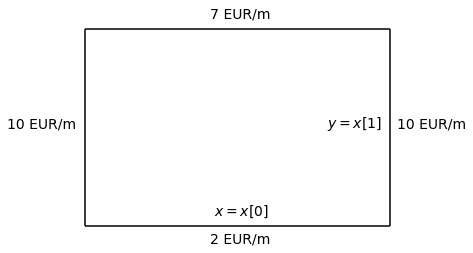
\includegraphics[width=0.4\textwidth]{figures/field.png}
\caption{Graphical representation of the \emph{field} minimization example.}
\label{fig:field}
\end{figure}

In this example there are two differences with respect to the previous:

\begin{itemize}
\tightlist
\item we want to \emph{maximize} a quantity (not minimize);
\item there is a constraint (we have a limited budget).
\end{itemize}

\pythoncodenon{code/bootstrap_6.py}

So let's repeat the steps as before. The objective is to maximize the enclosed area $A$ but our algorithm can only minimize functions. To overcome this issue 
the objective function can be defined to return the quantity $-A$, so that minimizing its value, the real objective, $A$, is maximized. 
Define length and width of the field respectively as \texttt{x[0]} and \texttt{x[1]} (items of the \texttt{list} \texttt{x}):

Then we can set the boundaries for length and width, their initial values (1~m each) and the other needed parameters.
Finally we have to impose the budget constraint. This is done by defining a function that computes the fence cost and compare it to the total budget. 
The constraint is passed to the minimizer as a dictionary (or a list  of dictionaries if there are more) which has three keys: \texttt{type}, in this case 
set to \texttt{'eq'} (like equality, since we want to spend all of our available money so the fence has to cost \textbf{exactly} 700~EUR), \texttt{'fun'} 
which defines the constraint function and \texttt{'args'} which is optional and set to a tuple whose items are the parameters for the constraint function 
(see Section~\ref{sec:kwargs_args}).

The constraint is then defined as
\begin{equation*}
\mathrm{budget} - \mathrm{fence~cost} = \mathrm{budget} - 2\cdot l\cdot\mathrm{side\_cost} - w\cdot(\mathrm{up\_cost} + \mathrm{down\_cost}) = 0
\end{equation*}

The optimization result tells us that the field has to be 17.5~m long and 38.9~m wide for a total field area of 680.5~$\textrm{m}^2$.

\subsection{Local Minima}
Minimization problems can be very nasty. For example when the objective function has various local minima, the parameter initial value choice can be critical. 
Assume we would like to minimize an objective function like 

\begin{equation*}
f(x) = \cfrac{\mathrm{cos}(3\pi x)}{x}
\end{equation*}
This function is plotted in Fig.~\ref{fig:local_minima} in the range $[0, 2]$, and clearly it has many minima. 

\begin{figure}[htb]
	\centering
	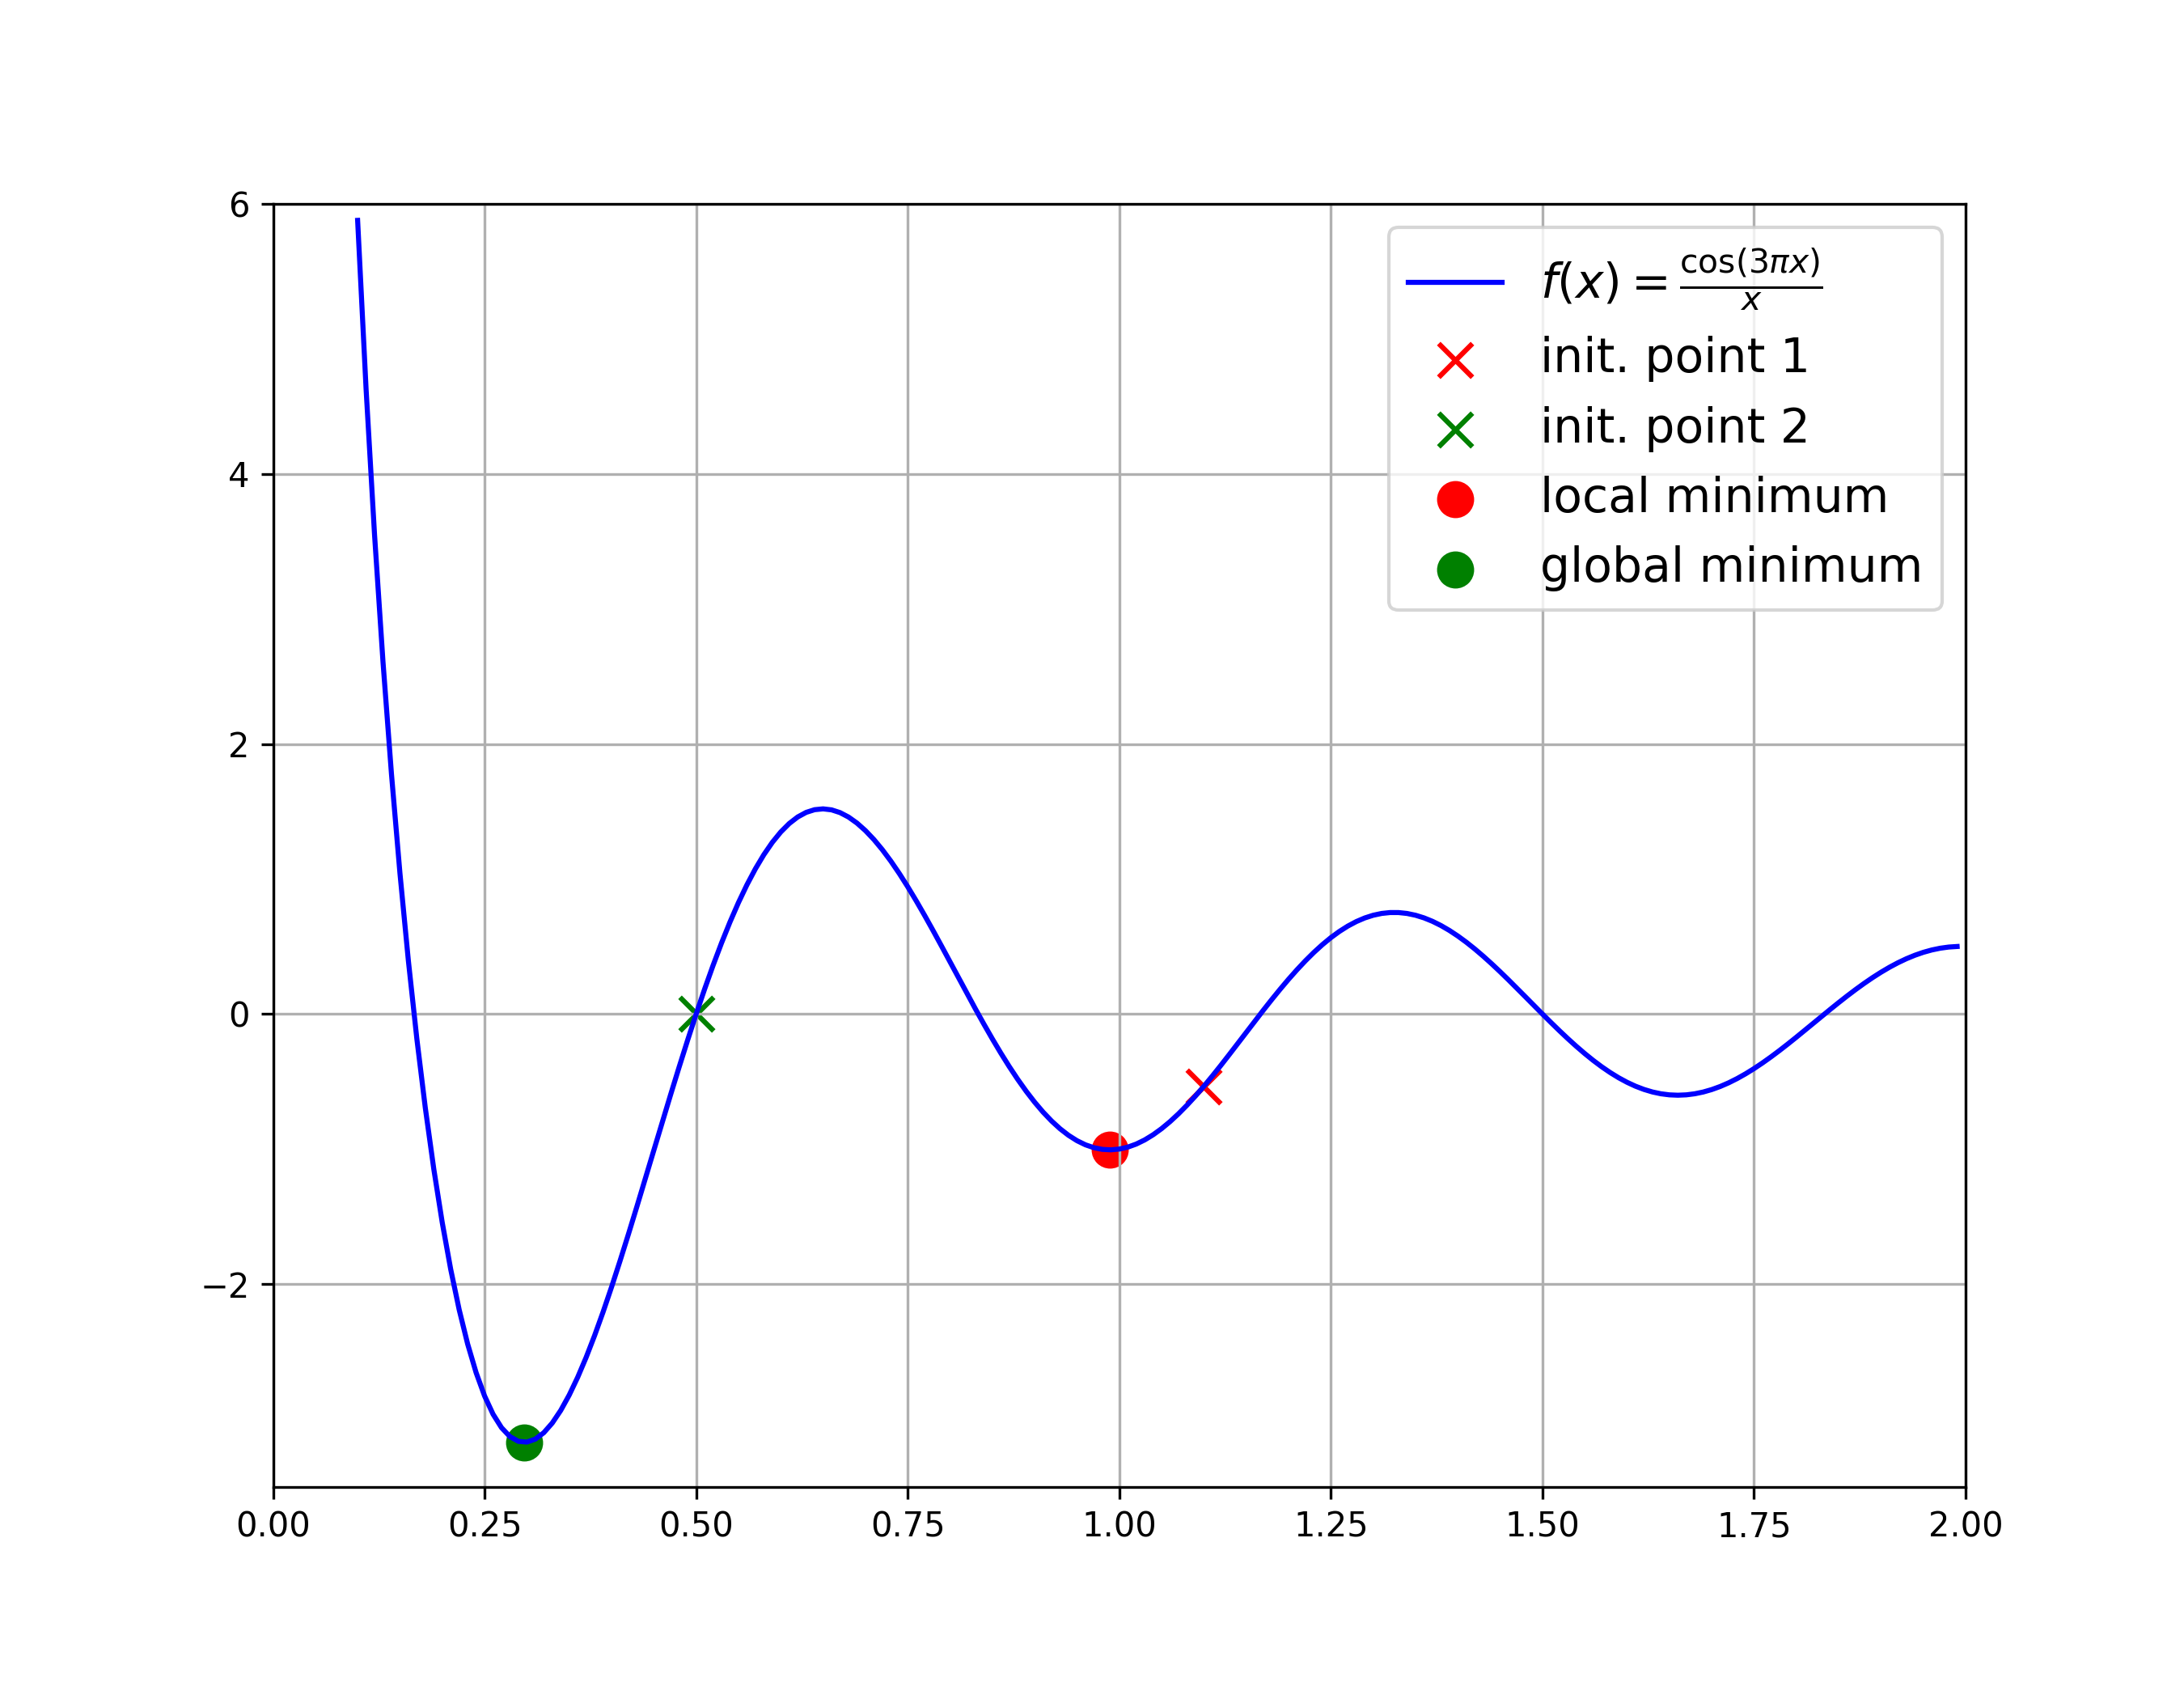
\includegraphics[width=0.7\textwidth]{figures/local_minima}
	\caption{Plot of an example function with many local minima. The red points highlights initial value and minimum found in a \emph{bad} minimization, green points for a good minimization.}
	\label{fig:local_minima}
\end{figure}
Let's try to find a minimum setting the initial value to $x=1.1$.
\begin{ipythonnon}
x0 = [1.1]
bounds = [(0.01, 20)]
r = minimize(func, x0, bounds=bounds)

print (r)
\end{ipythonnon}
\begin{ioutput}
     fun: array([-1.00569871])
hess_inv: <1x1 LbfgsInvHessProduct with dtype=float64>
     jac: array([-4.4408921e-07])
 message: b'CONVERGENCE: NORM_OF_PROJECTED_GRADIENT_<=_PGTOL'
    nfev: 16
     nit: 5
  status: 0
 success: True
       x: array([0.98865633])
\end{ioutput}
The minimization worked perfectly and we found $x=0.98865633$ (i.e. the red point in Fig.~\ref{fig:local_minima}) but this is not the absolute minimum we 
were expecting to find. The problem arise since the algorithm, following the derivative direction, has got stuck in a local minimum without any possibility 
to jump out the well.

If we repeat the minimization using as initial value $0.5$ instead
\begin{ipythonnon}
x0 = [0.5]
bounds = [(0.01, 20)]
r = minimize(func, x0, bounds=bounds)

print (r)
\end{ipythonnon}
\begin{ioutput}
     fun: array([-3.17151711])
hess_inv: <1x1 LbfgsInvHessProduct with dtype=float64>
     jac: array([9.76996262e-07])
 message: b'CONVERGENCE: NORM_OF_PROJECTED_GRADIENT_<=_PGTOL'
    nfev: 16
     nit: 5
  status: 0
 success: True
       x: array([0.29691798])
\end{ioutput}
Now clearly the algorithm found the absolute minimum in $x=0.29691798$ (i.e. the green point in Fig.~\ref{fig:local_minima}) because there was no chance to 
find a local minimum during the iterations.

This is just an example of what could happen when minimizing a function. When dealing with complicated cases it is possible to make a \emph{scan} of the objective 
function to try to approximately determine where the global minimum is and choose suitable initial values of the guess parameters.
%However there shouldn't be such an issue in the application of the bootstrap algorithm since the function that is minimized is a sum of squared terms which 
%has no local minimum, just a global one (i.e. it is a hyper-parabola).

\section*{Exercises}
%\begin{question}
Consider two 5\% coupon paying bonds (par value of \euro{100}) with the clean market prices of \euro{99.50} and \euro{98.30} and having maturities of 6 months and 1 year respectively.
Determine the spot rate for the 6-month and 1-year bond.  
\end{question}

\begin{solution}
At the end of 6 months the first bond will pay a coupon of \euro{2.5} (= \euro{100} * 5\%/ 2) plus the principal amount (= €100) which sums up to 102.50. To
determine the 6M spot rate we can write the following equation, :

\[ \cfrac{102.5}{(1 + S_{6M}/2)} = 99.5\qquad\Rightarrow\qquad S_{6M} = 2 \cdot \Big( \cfrac{102.5}{99.5} - 1 \Big) =  6.03 \%\]

At the end of another 6 months the second bond will pay a coupon of €2.5
(= €100 * 5\% / 2) plus the principal amount (= €100) which sums up to
€102.50. The bond is trading at €98.30, therefore, the 1-year spot rate
\(S_{1y}\) can be calculated using \(S_{6M}\) as,

\[ \cfrac{2.5}{(1+S_{6M}/2)} + \cfrac{102.5}{(1 + S_{1y}/2)^{2}} = 98.30 \]

\[ \cfrac{102.5}{(1 + S_{1y}/2)^{2}} = 98.30 - \cfrac{2.5}{(1+0.03015)} \]

\[ (2 + S_{1y})^{2} = \cfrac{4\cdot102.5}{98.87317} = 4.276428 \]

\[ S_{1y}^{2} + 4\cdot S_{1y} - 0.276428 = 0 \]

\[ S_{1y} = -2 \pm \sqrt{4 + 0.276428} =\begin{cases}\text{\sout{-4.06795}} \\ 6.80\%\end{cases} \]

\end{solution}

\begin{question}
A small petroleum company owns two refineries. Refinery 1 costs \$20,000 per day to operate, and it can produce 400 barrels of high-grade oil, 300 barrels of medium-grade oil, and 200 barrels of low-grade oil each day. Refinery 2 is newer and more modern. It costs \$25,000 per day to operate, and it can produce 300 barrels of high-grade oil, 400 barrels of medium-grade oil, and 500 barrels of low-grade oil each day.
The company has orders totaling 25,000 barrels of high-grade oil, 27,000 barrels of medium-grade oil, and 30,000 barrels of low-grade oil. How many days should it run each refinery to minimize its costs and still refine enough oil to meet its orders?

\noindent\textbf{Hint:} you need to identify the unknown quantities (working days for each refinery) and set the constraints on the production of barrels. The objective is to minimize the costs. If you have multiple constraints you can define a list of dictionaries (one for constraint). Furthermore in this case the constraint is not \emph{equal to} but rather \emph{greater than} so you have to set \texttt{ineq} type.
\end{question}

\cprotEnv\begin{solution}
Let's implement the usual steps for a minimization. In this case our unknown are \texttt{x[0]} and \texttt{x[1]} the working days for each refinery. Then define the objective function with the production costs and three more functions, one for each oil-grade for the constraints.

\begin{ipython}
from scipy.optimize import minimize

def of(x):
    return 20000*x[0] + 25000*x[1]

def cons1(x):
    return 400*x[0] + 300*x[1] - 25000

def cons2(x):
    return 300*x[0] + 400*x[1] - 27000

def cons3(x):
    return 200*x[0] + 500*x[1] - 30000

cons = [{"type":"ineq", "fun":cons1},
        {"type":"ineq", "fun":cons2},
        {"type":"ineq", "fun":cons3}]
\end{ipython}
Set limits and initial values and run the minimizer.
\begin{ipython}
x0 = [10, 10]
bounds = [(0, 100) for _ in range(len(x0))]
r = minimize(of, x0, bounds=bounds, constraints=cons)
print (r)
\end{ipython}
\begin{ioutput}
     fun: 1750002.070622686
     jac: array([20000., 25000.])
 message: 'Optimization terminated successfully.'
    nfev: 8
     nit: 6
    njev: 2
  status: 0
 success: True
       x: array([25.00004033, 50.00005056])
\end{ioutput}    
So refinery 1 should work 25 days while refinery 2 50 days to minimize the production costs to 1750000 M (see objective function value in the minimization report).
\end{solution}

\begin{question}
Read the OIS market data from \href{https://drive.google.com/file/d/1LCEDmheKqwPXFpJ25hFz32QI5im2UJO1/view?usp=sharing}{\texttt{ois\_data.xlsx}} and, using the \texttt{OvernightIndexSwap} class,construct the corresponding swaps.
\end{question}

\cprotEnv\begin{solution}

\begin{ipython}
import pandas, datetime
from finmarkets import OvernightIndexSwap, generate_swap_dates

observation_date = datetime.date.today()
df = pandas.read_excel('ois_data.xlsx')

market_quotes = {}
for i in range(len(df)):
    key = df.loc[i, 'months']
    value = df.loc[i, 'quote']
    market_quotes[key] = value

swaps = []
for months, rate in market_quotes.items():
    swap = OvernightIndexSwap(1e6,
        generate_swap_dates(observation_date, months),
        0.01 * rate)

swaps.append(swap)
\end{ipython}
\end{solution}

\begin{question}
From the \texttt{OvernightIndexSwap} created in the previous example derive a discount curve using the bootstrap method.
\end{question}

\cprotEnv\begin{solution}
We have just created some swaps from the market quotes in the previous exercise, so now we can just create a list with the pillar dates.

\begin{ipython}
observation_date = date(2019, 10, 23)
pillar_dates = [observation_date]

for swap in swaps:
    pillar_dates.append(swap.payment_dates[-1])

# this shouldn't be necessary if the original
# list of market quotes is sorted
pillar_dates = sorted(pillar_dates)
\end{ipython}
Define the objective function: the sum of the squared NPVs of the OIS.
\begin{ipython}
def objective_function(x):
    curve = DiscountCurve(observation_date,
        pillar_dates, x)

    sum_sq = 0.0
    for swap in swaps:
        sum_sq += swap.npv(curve) ** 2
    return sum_sq
\end{ipython}
Set the initial value of the discount factors (\(x_i\)) to 1 with a range of variability \([ 0.01, 10]\), in addition the first element of the list, today's discount factor, will be fixed to 1 (variability \([1, 1]\)).

\begin{ipython}
x0 = [1.0 for i in range(len(pillar_dates))]

bounds = [(0.01, 10.0) for i in range(len(pillar_dates))]
bounds[0] = (1.0, 1.0)
\end{ipython}
Finally launch the minimizer to find the discount factors (\(\mathbf{x}\)).

\begin{ipython}
from scipy.optimize import minimize

result = minimize(objective_function, x0, bounds=bounds)
print (result)
\end{ipython}
\begin{ioutput}
     fun: 0.000819919032900304
hess_inv: <34x34 LbfgsInvHessProduct with dtype=float64>
     jac: array([ 6.58948735e+05, -1.58720803e+01, -6.53143264e+01, 
                 -1.03323232e+02, -1.26050260e+02, -1.31748898e+02, 
                 -1.20374599e+02, -9.15399651e+01, -4.24363322e+01,  
                  2.44903182e+01,  1.14345243e+02,  2.22002243e+02,
                 -3.72021700e+00,  4.21398633e+01,  4.21787852e+01,  
                  4.22369487e+01,  4.23327026e+01,  4.31814758e+01,  
                  4.44924460e+01,  4.62078978e+01,  4.82906823e+01, 
                  -3.69972738e+00,-1.42454702e+00,  7.53771932e-01,
                  2.79741018e+00,  4.62896699e+00,  6.24844054e+00,  
                  9.93101553e+00,  1.31122434e+01,  1.42880909e+01,  
                  1.48279215e+01,  1.50787019e+01,  1.43267935e+01,  
                  1.38451324e+01])
 message: b'CONVERGENCE: REL\_REDUCTION\_OF\_F\_<=\_FACTR*EPSMCH'
    nfev: 840
     nit: 7
  status: 0
 success: True
       x: array([1.        , 1.00030147, 1.00058831, 1.00089012, 1.00119726,
                 1.00147996, 1.00178743, 1.00208107, 1.00238467, 1.00267865,
                 1.00298261, 1.00327737, 1.00357104, 1.00357104, 1.00355063,
                 1.00352002, 1.00346901, 1.00302007, 1.00232627, 1.00141821,
                 1.00031629, 0.99911234, 0.99790839, 0.99675545, 0.99567393,
                 0.99470465, 0.9938476 , 0.99189884, 0.99021534, 0.98959296,
                 0.98930728, 0.98917464, 0.98957256, 0.98982763])
\end{ioutput}
\end{solution}

%\begin{question}
%Take the \texttt{OvernightIndexSwap} class from \texttt{finmarkets} module and add a new method called \texttt{fair\_value\_strike} which takes a discount curve object and returns the fixed rate which would make the OIS with zero NPV.
%
%\noindent\textbf{Hint:} first take the formulas for the NPV of the fixed and floating legs, put one equal to the other and solve for $K$.
%\end{question}
%
%\cprotEnv\begin{solution}
%As the hint suggested the two NPV equations are compared:
%
%\[\mathrm{NPV}_{\mathrm{fix}} = NK \sum_{i=1}^{n}D(d_{i})\cfrac{d_i - d_{i-1}}{360}\]
%
%\[\mathrm{NPV}_{\mathrm{float}} = N \cdot [D(d_0) - D(d_n)]\]
%
%\[K \sum_{i=1}^{n}D(d_{i})\cfrac{d_i - d_{i-1}}{360} = [D(d_0) - D(d_n)]\]
%
%\[K = \cfrac{[D(d_0) - D(d_n)]}{\sum_{i=1}^{n}D(d_{i})\cfrac{d_i - d_{i-1}}{360}}\]
%Now in \texttt{python}:
%
%\begin{ipython}
%class OverNightIndexSwap:
%    ...
%    def fair_value_strike(self, discount_curve):
%        den = 0
%        for i in range(1, len(self.payment_dates)):
%            start_date = self.payment_dates[i-1]
%            end_date = self.payment_dates[i]
%            tau = (end_date - start_date).days / 360
%            df = discount_curve.df(end_date)
%            den += df * tau
%            num = (discount_curve.df(self.payment_dates[0]) -
%                discount_curve.df(self.payment_dates[-1]))
%        return num/den
%\end{ipython}
%Finally add this method to the class implementation in \texttt{finmarkets.py}.
%\end{solution}

